\documentclass[8pt]{beamer} %[handout]
\usepackage[utf8]{inputenc}
%\usepackage[italian]{babel}

\usepackage{amsmath}
\usepackage{amssymb}
\usepackage{amsthm}
\usepackage{mathtools}
\usepackage{mwe}
\usepackage{listings}
\usepackage{multicol}
% \usepackage{beton}
% \usepackage{euler}
% \usepackage{fontspec}
\usepackage[T1]{fontenc}
\usepackage{xcolor}
\setlength{\marginparwidth}{1.5cm}
\usepackage{verbatim}

\usepackage[doi=false, url=false]{biblatex}
\usepackage{csquotes}
\usepackage[makeroom]{cancel}
\addbibresource{./bibliography.bib}

\title{\Huge{Generalization of NLIN model\\ for WDM systems}}
\date{}


\titlegraphic{
\includegraphics[width=0.15\textwidth]{./images/logo/unipd-text.png} \hspace{1cm} 
\includegraphics[width=0.15\textwidth]{./images/logo/DEI-text.png}}

\usetheme{Berlin}
\usecolortheme{beaver}
% \usefonttheme{structuresmallcapsserif}
\usepackage{textpos}
%\addtobeamertemplate{frametitle}{}{%
%\begin{textblock*}{100mm}(.85\textwidth,-1.1cm)
%\hspace{1cm}
\includegraphics[width = 0.2cm]{../images/logo/DEI.png}
%\end{textblock*}}
\usefonttheme{professionalfonts} % using non standard fonts for beamer
\usefonttheme{serif} % default family is serif
% remove navigation symbols from beamer theme
\beamertemplatenavigationsymbolsempty

% \addtobeamertemplate{navigation symbols}{}{
%   \usebeamerfont{footline}
%   \usebeamercolor[fg]{footline} 
%   \hspace{1em}
%   \insertframenumber/\inserttotalframenumber
% }

\setbeamertemplate{footline}{}
%\setbeamertemplate{caption}{\raggedright\insertcaption\par}

  

\begin{document}

\begin{frame}
  \maketitle
\end{frame}

\begin{frame}
  \frametitle{}
  \Huge{Computation of integrals and \\survey on feasible approximations}
  \vspace{30pt}
  \normalsize{
  \begin{itemize}
  	\item Numerical convergence of time integrals
  	\item Numerical convergence of space integrals
  	\item Insights on Papoulis approximation
  	\item Correction term for Gaussian pulses space integrals
  \end{itemize}

}
\end{frame}

\begin{frame}
  \frametitle{Integral of interest}
	\begin{equation}
		X_{0, m, m} = \int_{0}^{L} dz f_B(z) \int_{-\infty}^{\infty} dt\, |g^{(0)}(z, t)|^2 \,|g^{(0)}(z, t-mT -\beta_2 \Omega z)|^2
	\end{equation}
	in the following the perfect amplification approximation is used
	\begin{equation}
		f_B(z) = 1
	\end{equation}
\end{frame}

\begin{frame}
	\frametitle{}
	\huge{Convergence of \textit{time} integrals \\for various pulse shapes}
	\vspace{30pt}
	
	\normalsize{All computations are done using 40 points per collision in space integral}
\end{frame}

\begin{frame}
	
	\frametitle{Nyquist (sinc) pulses - time steps evaluation}
	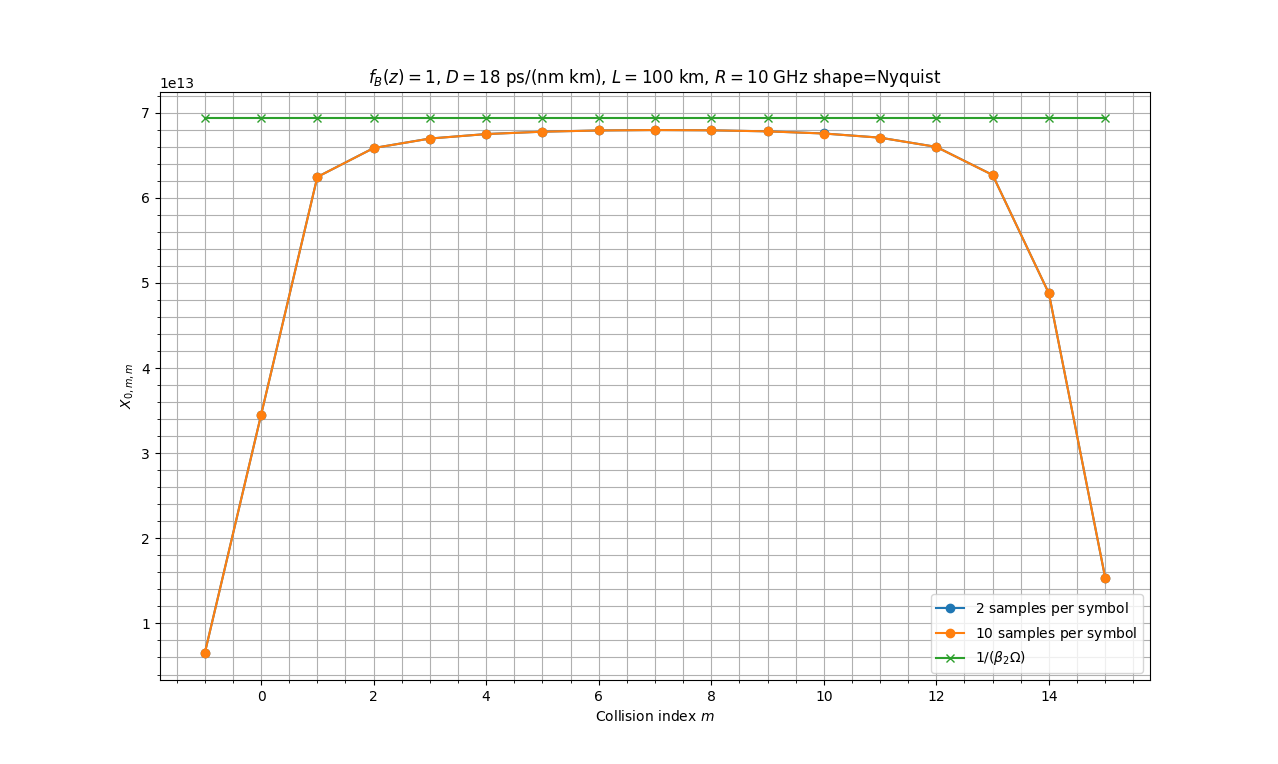
\includegraphics[width=\textwidth]{"./images/sim/Nyquist_time.png"}
\end{frame}

\begin{frame}
	\frametitle{Raised cosine pulses - time steps evaluation}
	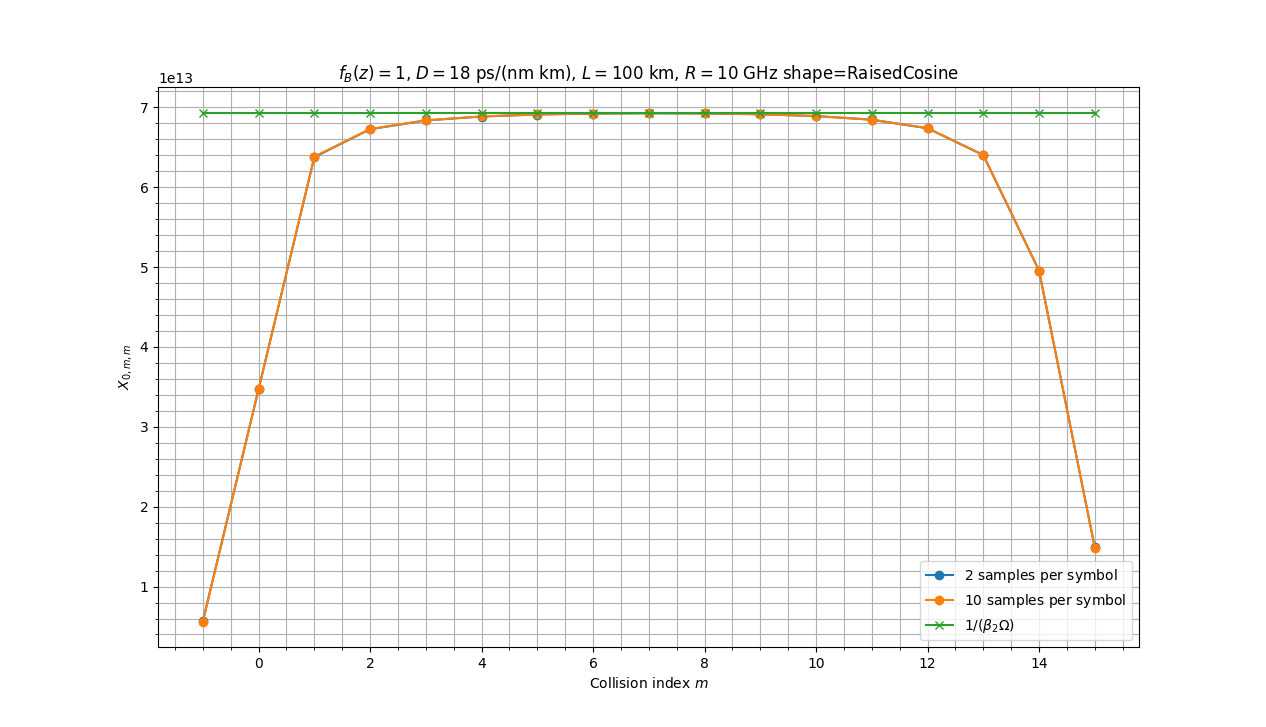
\includegraphics[width=\textwidth]{"./images/sim/Raised_time.png"}
\end{frame}

\begin{frame}
  \frametitle{Gaussian pulses - time steps evaluation}
  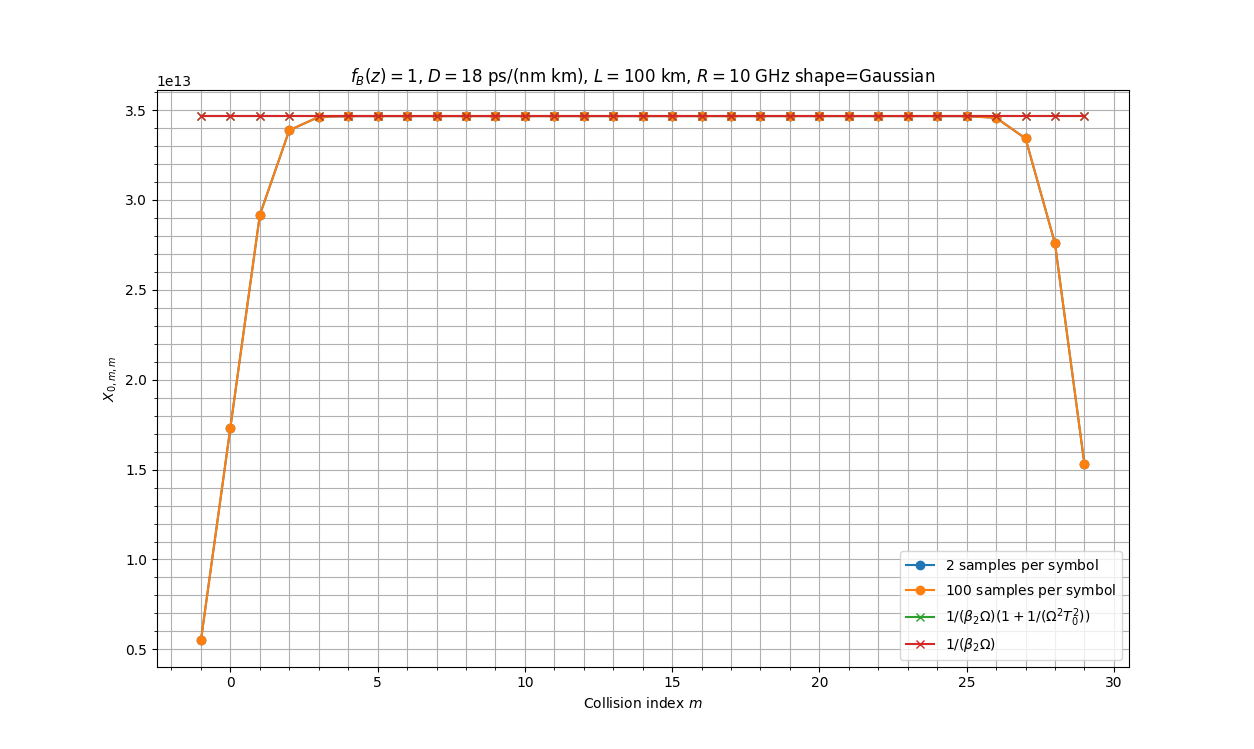
\includegraphics[width=\textwidth]{"./images/sim/very much.png"}
\end{frame}

\begin{frame}
	\frametitle{}
	\huge{Convergence of \textit{space} integrals \\for various pulse shapes}
	
		\vspace{30pt}
	\normalsize{All computations are done using 10 samples per symbol in time integral}
\end{frame}


\begin{frame}
	\frametitle{Nyquist (sinc) pulses - space steps evaluation}
	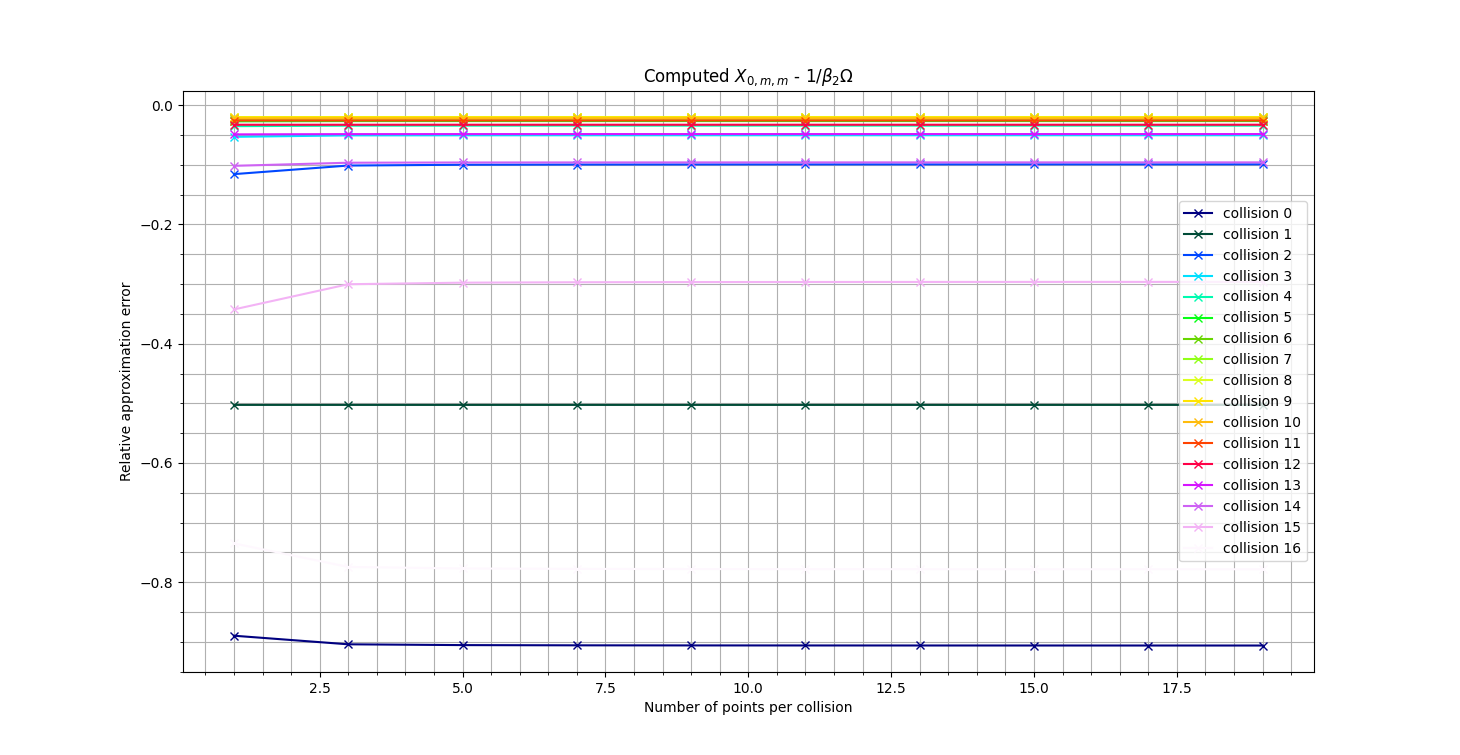
\includegraphics[width=\textwidth]{"./images/sim/spatial_collision_N.png"}
\end{frame}

\begin{frame}
	\frametitle{Nyquist (sinc) pulses - space steps evaluation}
	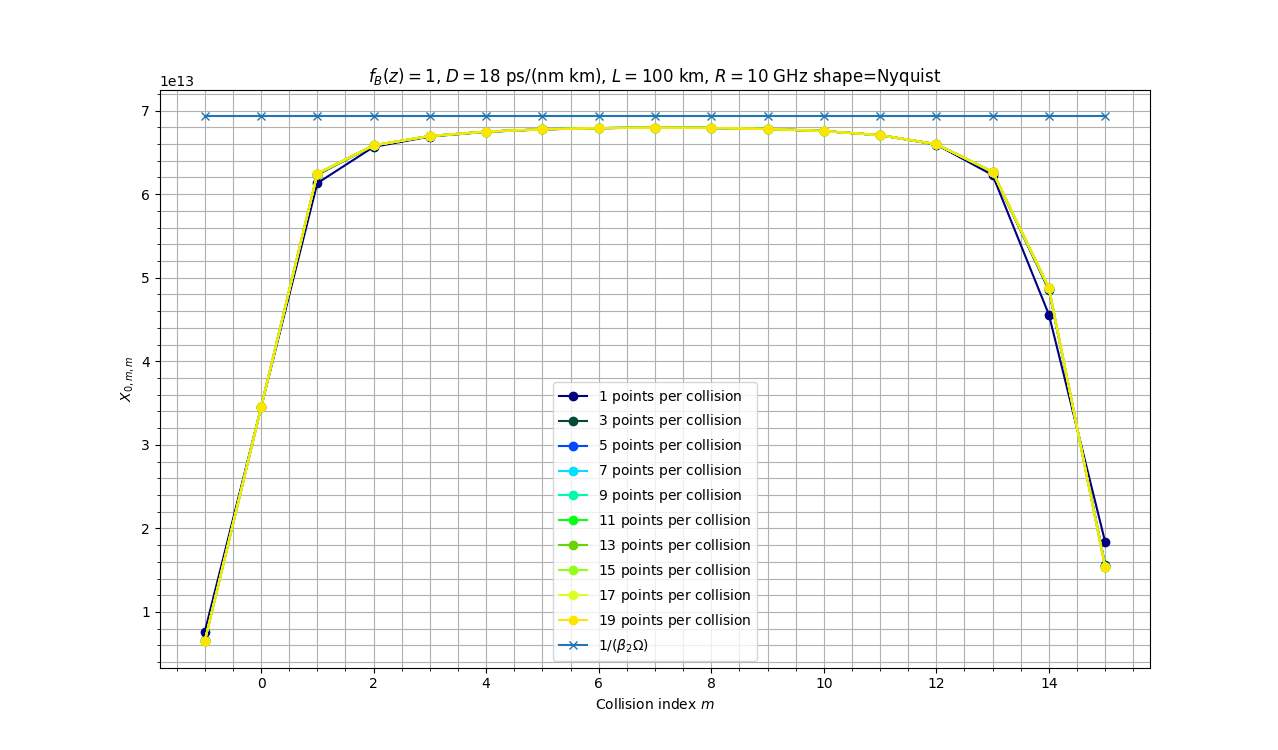
\includegraphics[width=\textwidth]{"./images/sim/spatial_N.png"}
\end{frame}

\begin{frame}
	\frametitle{Raised cosine pulses - space steps evaluation}
	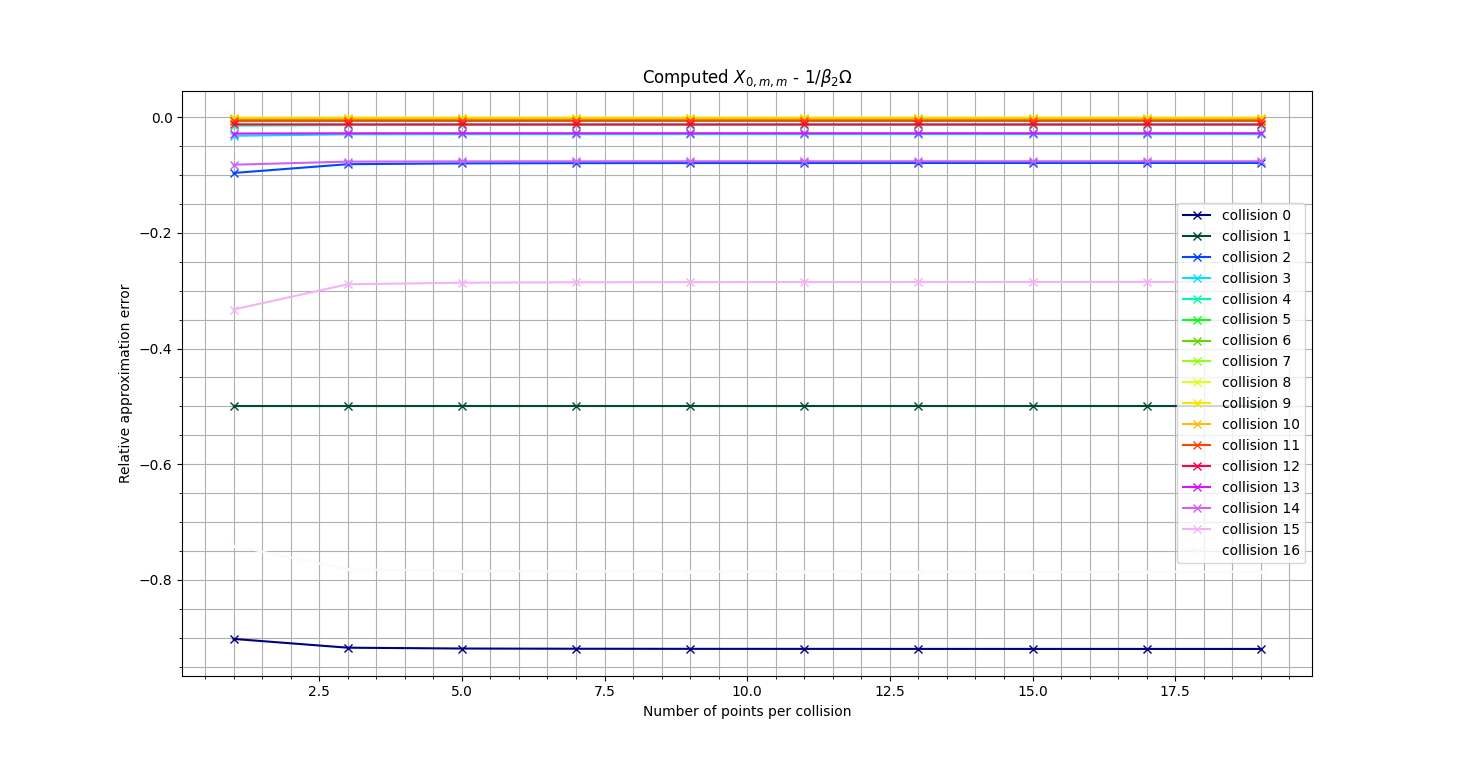
\includegraphics[width=\textwidth]{"./images/sim/spatial_collision_RC.png"}
\end{frame}

\begin{frame}
	\frametitle{Raised cosine pulses - space steps evaluation}
	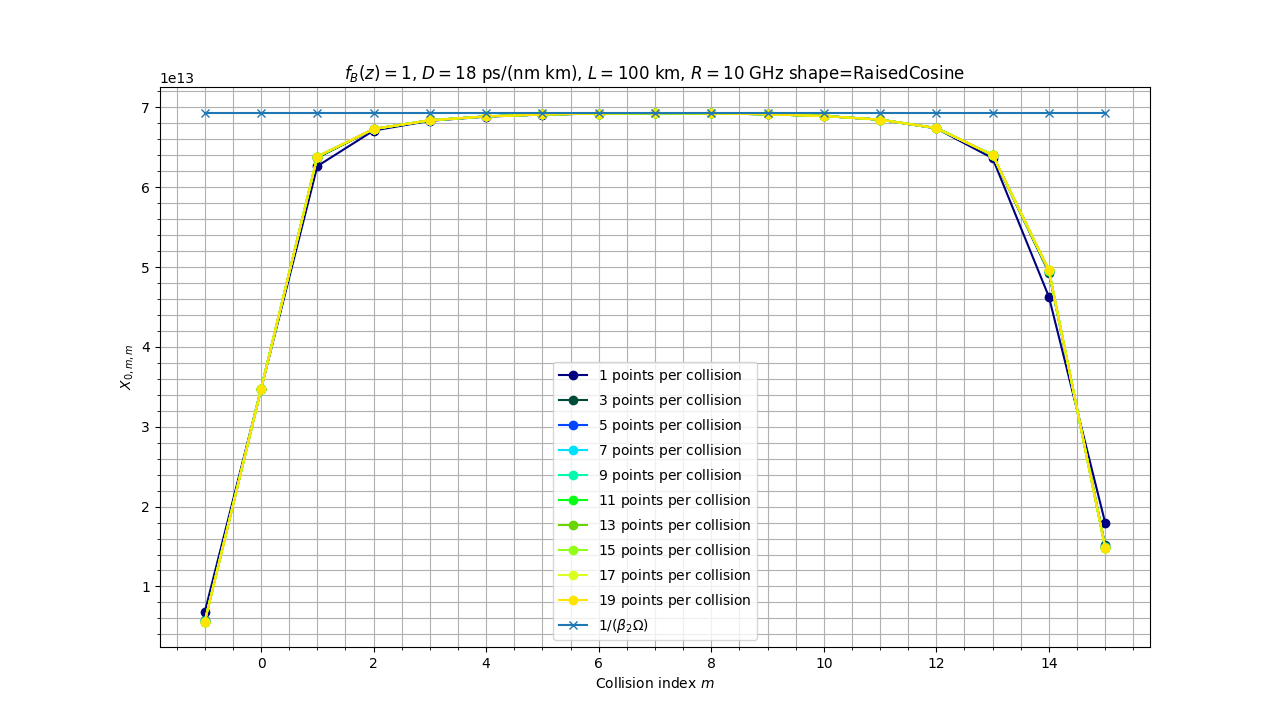
\includegraphics[width=\textwidth]{"./images/sim/spatial_RC.png"}
\end{frame}

\begin{frame}
	\frametitle{Gaussian pulses - space steps evaluation}
	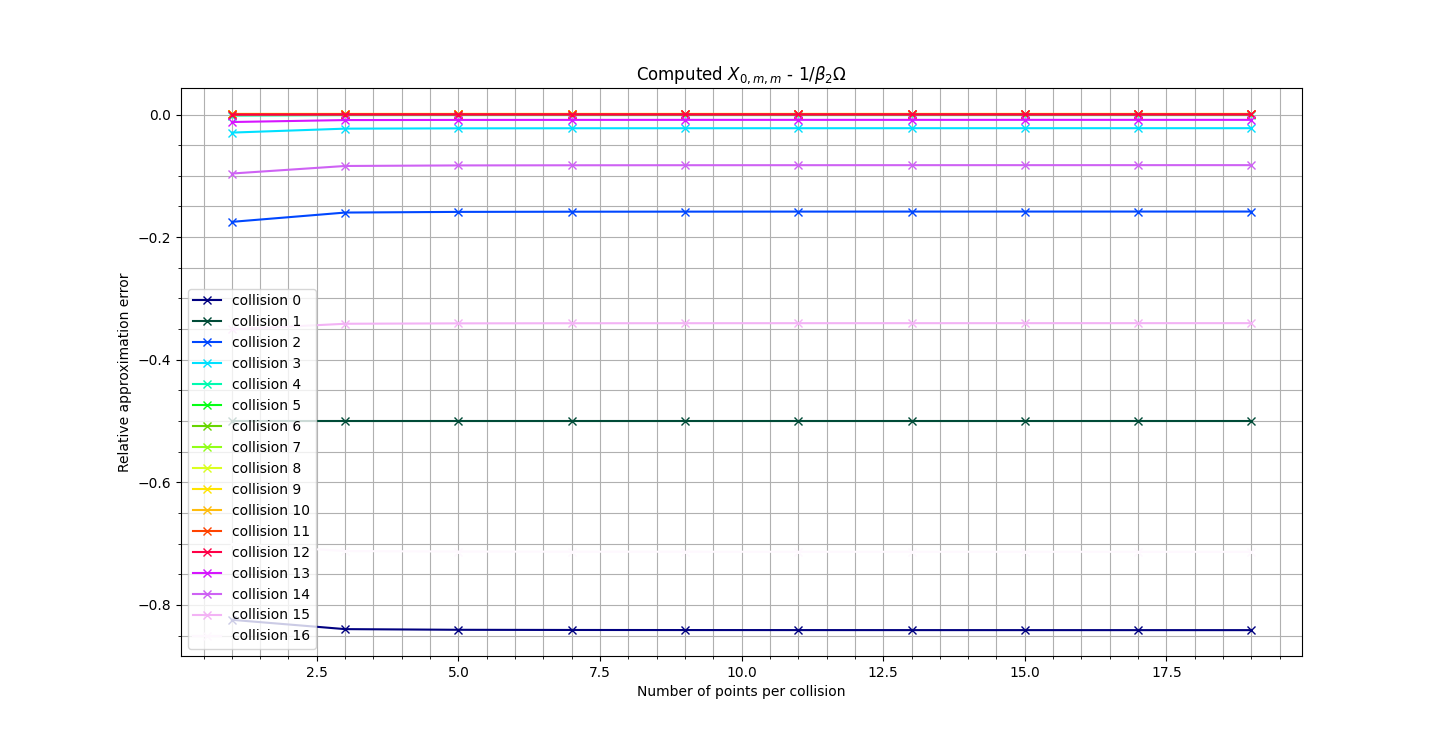
\includegraphics[width=\textwidth]{"./images/sim/spatial_collision_G.png"}
\end{frame}

\begin{frame}
	\frametitle{Gaussian pulses - space steps evaluation}
	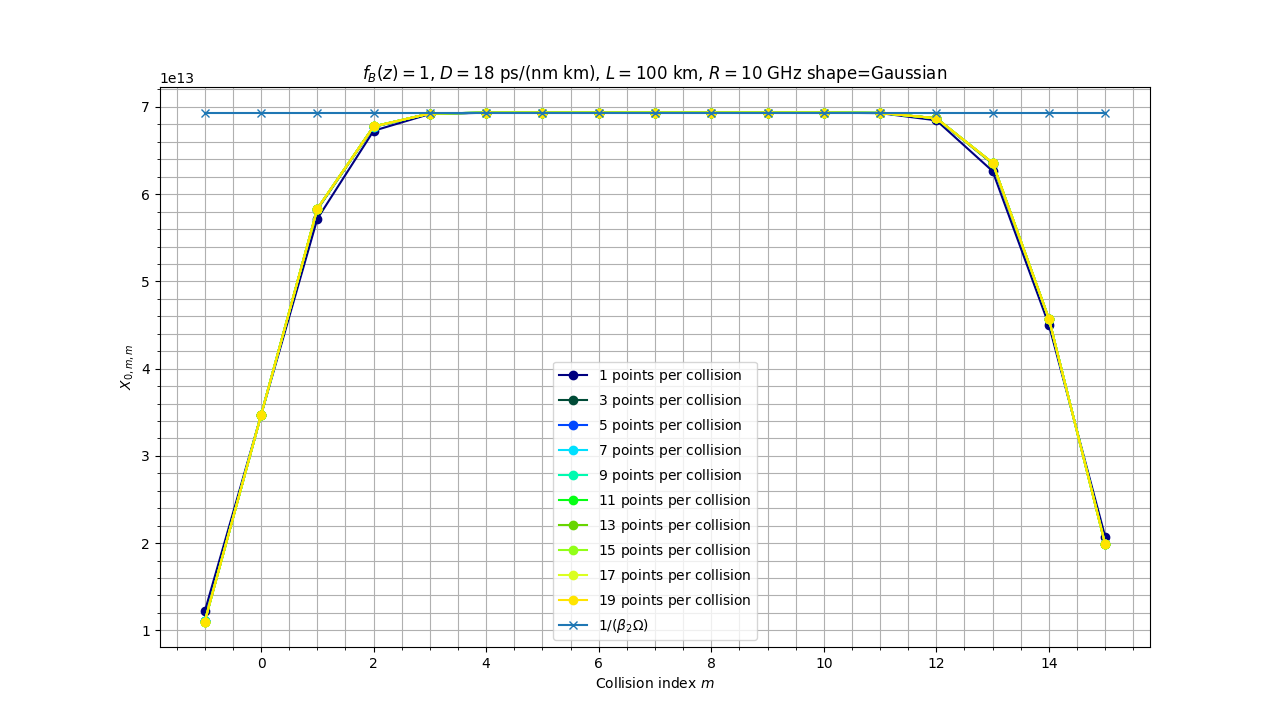
\includegraphics[width=\textwidth]{"./images/sim/spatial_G.png"}
\end{frame}


\begin{frame}
	\frametitle{Approximation using Fresnel transform (Papoulis)}
	The approximation from \cite{Papoulis_1994} relates the propagated pulse shape with its Fourier transform
	\begin{equation}
		g^{(0)}(z, t)=\sqrt{\frac{i}{2 \pi \beta_{2} z}} \exp \left[-\frac{i t^{2}}{2 \beta_{2} z}\right] \hat{g}\left(0, \frac{t}{\beta_{2} z}\right)
	\end{equation}
	This is derived using the system function properties of the fiber linear propagator operator.
	In spectral domain the operator reads
	\begin{equation}
		\hat{U}(z)=\exp \left[-i \frac{\beta_{2}}{2} z \omega^{2}\right]
	\end{equation}
	and using the Gaussian transform relation
	\begin{equation}
		\exp \left[-s t^{2}\right] \longleftrightarrow \sqrt{\frac{\pi}{s}} \exp \left[-\frac{\omega^{2}}{4 s}\right]
	\end{equation}
	we can find a convolution kernel
	\begin{equation}
		\hat{U}(z)=\exp \left[-i \frac{\beta_{2}}{2} z \omega^{2}\right] \longleftrightarrow U(z, t)=\sqrt{\frac{-i}{2 \beta_{2} z \pi}} \exp \left[i \frac{t^{2}}{2 \beta_{2} z}\right]
	\end{equation}
\end{frame}

\begin{frame}
	\frametitle{Quadratic Phase Filter}
	The linear propagation corresponds to a convolution operation by this kernel. Since the frequency response denotes a quadratic phase term, the corresponding filter is called Quadratic Phase Filter.
	The convolution is actually well-known, and it assumes the shape of a Fresnel transform.
	\begin{equation}
		\bar{f}(t)=\sqrt{\frac{\beta}{i \pi}} \int_{\mathbb{R}} f(\tau) \exp \left[-i \beta(t-\tau)^{2}\right] d \tau
	\end{equation}
Starting from the Fresnel transform, a \textit{square completion argument} links the propagated field to its Fourier transform.

A comprehensive derivation presentation will soon be added.
\end{frame}


\begin{frame}
  \frametitle{Gaussian pulses}
  Substituting the Gaussian pulse shape in the XPM coefficient definition we obtain, using a change of \textit{time} variable
  \begin{equation}
    X_{0, m, m}=\frac{1}{\sqrt{2}} \int_{0}^{L} d z \frac{U_{0}^{4}}{1+D^{2}(z)} \exp \left[-\frac{\left(m T+\beta_{2} \Omega z\right)^{2}}{2 T_{0}^{2}\left(1+D(z)^{2}\right)}\right] \int_{\mathbb{R}} d \eta \exp \left[-\frac{\eta^{2}}{T_{0}^{2}\left(1+D(z)^{2}\right)}\right]
  \end{equation}
where $D = \dfrac{z}{L_D} = z \dfrac{\beta_2}{T_0^2}$.
The time integral admits an analytic solution
  \begin{equation}
    X_{0, m, m}=\frac{1}{\sqrt{2}} \int_{0}^{L} d z \frac{\sqrt{\pi} U_{0}^{4} T_{0} \sqrt{1+D(z)^{2}}}{1+D(z)} \exp \left[-\frac{\left(m T+\beta_{2} \Omega z\right)^{2}}{2 T_{0}^{2}\left(1+D(z)^{2}\right)}\right]
  \end{equation}
\end{frame}

\begin{frame}
  \frametitle{Space integral}
  The space integral can be simplified to express a space-dependent Gaussian width $\sigma=T_{0}\sqrt{1+D^{2}}$. Extending to the whole space, 
  \begin{equation}
    X_{0, m, m}=\sqrt{\pi} U_{0}^{4} T_{0}^{2} \int_{\mathbb{R}} d z \frac{1}{\sqrt{2} T_{0} \sqrt{1+D(z)^{2}}} \exp \left[-\frac{\left(m T+\beta_{2} \Omega z\right)^{2}}{2 T_{0}^{2}\left(1+D(z)^{2}\right)}\right]
  \end{equation}
and adopting a change of variable
  \begin{equation}
    X_{0, m, m}=\frac{\sqrt{\pi} U_{0}^{4} T_{0}^{2}}{\beta_{2} \Omega} \int_{\mathbb{R}} d\zeta \frac{1}{\sqrt{2} T_{0} \sqrt{1+D^{2}}} \exp \left[-\frac{(\zeta+m T)^{2}}{2 T_{0}^{2}\left(1+D^{2}\right)}\right]
  \end{equation}
in the last integral, with a slight abuse of notation $D = D(\zeta)$.

Remember the normalization condition
\begin{equation}
	\pi U_{0}^{4} T_{0}^{2} = 1
\end{equation}
\end{frame}

\begin{frame}
	\frametitle{Local interaction ($0^{th}$-order) approximation}
	As proven in the previous computation, a local interaction approximation is useful when $D(z) \approx D_m := D(z_m)$, with $z_m = -\dfrac{mT}{\beta_2 \Omega}$.
	In this case, the time integral is a simple Gaussian integral, and it can be evaluated as
	\begin{equation}
		X_{0, m, m} = \dfrac{1}{\beta_2 \Omega}
	\end{equation}
	this approximation is not useful for Nyquist and raised cosine pulses, and a slight improvement is available for Gaussian integrals.
\end{frame}

\begin{frame}
	\frametitle{Correction to the $0^{th}$-order approximation}
	By expanding the dependence on $D$ to the second order, around $D_m$, we obtain a correction which accounts for the dispersion phenomenon \textit{inside} the relevant collision region
	\begin{equation}
		X_{0, m, m} \approx X_{0, m, m}^{(0)} + \Delta X_{0, m, m}^{(2)}
	\end{equation}
	where 

	\begin{equation}\label{eq:correction}
	\Delta X_{0, m, m}^{(2)} = \dfrac{1}{\beta_2 \Omega} \dfrac{1}{\Omega^2 T_0^2}
	\end{equation}
	the corrected coefficient reads
	\begin{equation}
		X_{0, m, m} \approx \dfrac{1}{\beta_2 \Omega} \left(1+\dfrac{1}{\Omega^2 T_0^2}\right)
	\end{equation}
this correction is well verified by numerical computation of the integral.
\end{frame}


\begin{frame}
  \frametitle{First order correction}
  In order to simplify the computation we use a change of variable
  \begin{equation}
    \frac{d \sigma}{d D}=\left(-T_{0} \frac{D_{m}}{\sqrt{1+D_{m}^{2}}}\right)
  \end{equation}
By using the rule for computing Gaussian moments we have
  \begin{align}
    \Delta X_{0, m m}^{(1)} & =\frac{\sqrt{\pi} U_{0}^{4} T_{0}^{2}}{\beta_{2} \Omega} \int_{\mathbb{R}} d \zeta \frac{\partial C}{\partial D}\left(D_{m}, \zeta\right) \cdot\left(D-D_{m}\right)=                                                                                          \\
                            & =\frac{\sqrt{\pi} U_{0}^{4} T_{0}^{2}}{p_{2} \Omega} \int_{\mathbb{R}} d\zeta \frac{1}{\sqrt{2} \sigma_{m}} \cdot \exp \left[-\frac{(\zeta+m T)^{2}}{2 \sigma_{m}^{2}}\right] \left[-\frac{1}{\sigma_{m}}+\frac{(\zeta+m T)^2}{\sigma_{m}^{3}}\right]  \times \\
                            & \times \left[-T_{0} \frac{D_{m}}{\sqrt{1+D_{m}^{2}}}\right] \cdot\left(\frac{\zeta+m T}{\Omega T_{0}^{2}}\right) = 0
  \end{align}
as the only moments occuring are mean and kurtosis.
\end{frame}

\begin{frame}
  \frametitle{Second order correction (1)}
  	Let us use the chain rule twice
  \begin{equation}\label{eq:sum}
  	\frac{\partial^{2} C}{\partial D^{2}}=\frac{d^{2} \sigma}{d D^{2}} \cdot \frac{\partial C}{\partial \sigma}+\left(\frac{d \sigma}{d D}\right)^{2} \frac{\partial^{2} C}{\partial \sigma^{2}}
  	\end{equation}
  	By integrating the first term of the sum in eq (\ref{eq:sum}) we obtain

\begin{align}
	\frac{\sqrt{\pi} U_{0}^{4} T_{0}^{2}}{\beta_{2} \Omega} &\int_{\mathbb{R}} d \zeta \frac{1}{\sqrt{2} \sigma_m} \exp \left[-\frac{\left(\zeta+m T\right)^{2}}{2 \sigma_m^{2}}\right] \left[-\frac{1}{\sigma_{m}}+\frac{(\zeta+m T)^2}{\sigma_{m}^{3}}\right] \times\\
	\\ & \times  \,   \left[ \frac{T_0}{\left({1+D_{m}^{2}}\right)^{3/2}}\right] \, \frac{1}{2} \frac{(\zeta+m T)^{2}}{\Omega^{2} T_{0}^{4}}
\end{align}
so we have a variance, and a central moment of order 4.
\end{frame}

\begin{frame}
	\frametitle{Second order correction (2)}
	As for the second term in \ref{eq:sum} the integral reads
	\begin{align}
		=\frac{\sqrt{\pi} U_{0}^{4} T_{0}^{2}}{\beta_{2} \Omega} &\int_{\mathbb{R}} d \zeta \frac{1}{\sqrt{2} \sigma_m} \exp \left[-\frac{\left(\zeta+m T\right)^{2}}{2 \sigma_m^{2}}\right]\left[\left(-\frac{1}{\sigma_m}+\frac{\left(\zeta+m T\right)^{2}}{\sigma_m^{3}}\right)^{2}+\right.\\
		\\ & \left.+\left(\frac{1}{\sigma_m^{2}}-\frac{3(\zeta+m T)^{2}}{\sigma_m^{4}}\right)\right] \, \left(-T_{0} \frac{D_{m}}{\sqrt{1+D_{m}^{2}}}\right)^{2} \, \frac{1}{2} \frac{(\zeta+m T)^{2}}{\Omega^{2} T_{0}^{4}}
	\end{align}
	so we have a variance, and central moments of order 4 and 6.
	Using the rule
	\begin{equation}
		\mathbb{E}[(X-\mu)^n] = (n-1)!! \sigma^n
	\end{equation}
we obtain the integrals.\\
	Summing the two contribution the dependence on $D_m$ vanishes, and we are left with eq. (\ref{eq:correction})
\end{frame}

\begin{frame}
	\frametitle{Second order correction}
	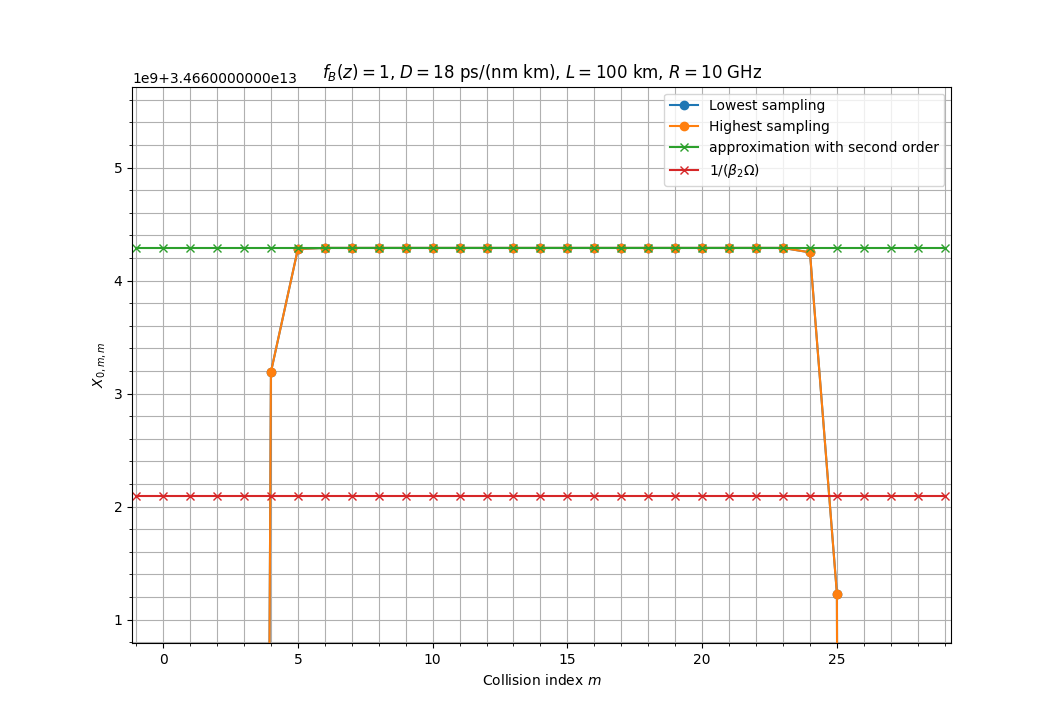
\includegraphics[width=\textwidth]{"./images/sim/second_order.png"}
\end{frame}

\begin{frame}
	\frametitle{}
	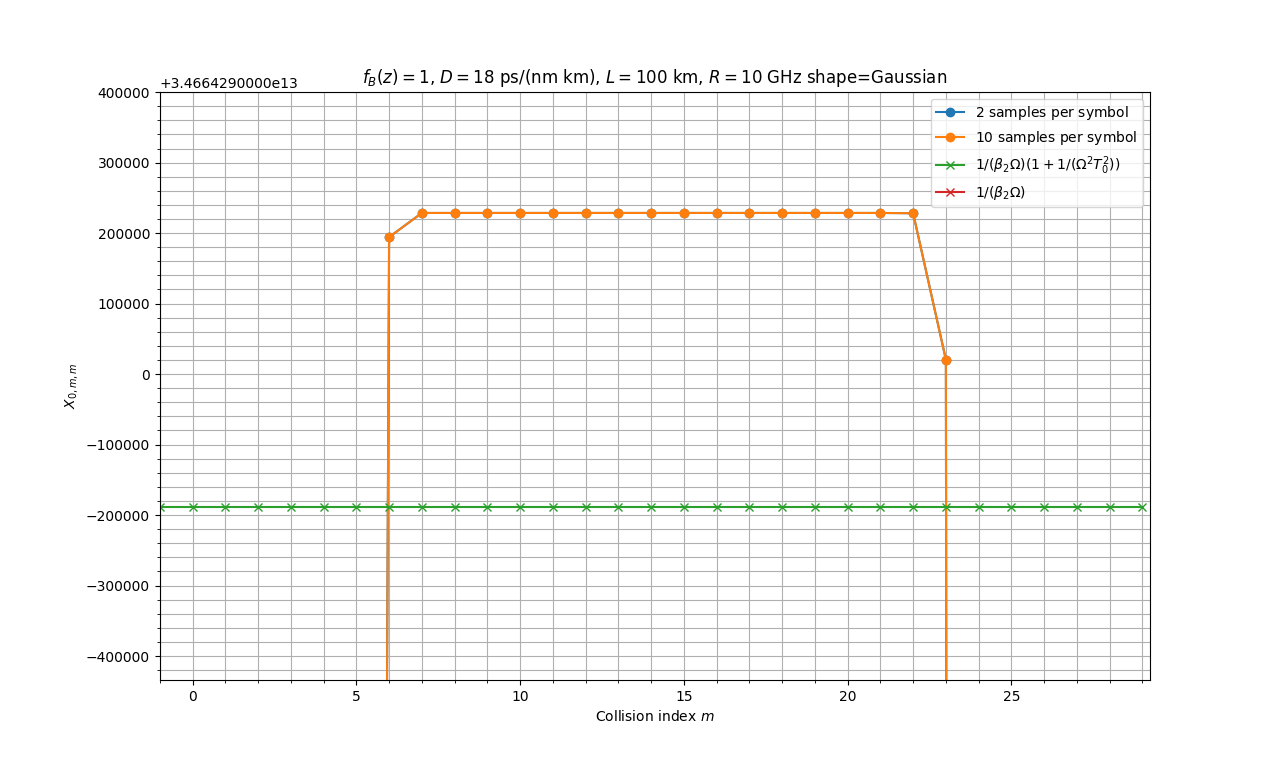
\includegraphics[width=\textwidth]{"./images/sim/second_error.png"}
\end{frame}

\end{document}